\section{Arquitetura de Microsserviços}

A arquitetura de microsserviços é um estilo de desenvolvimento de software que estrutura uma aplicação como uma coleção de serviços pequenos, autônomos e fracamente acoplados. A premissa central consiste em decompor um sistema complexo em componentes independentes, nos quais cada serviço é responsável por uma capacidade de negócio específica e pode ser desenvolvido, implantado e escalado de forma autônoma \cite{newman_building_2022,fowler_microsservicos_2022}.

Essa modularidade permite que equipes atuem em paralelo, utilizando tecnologias adequadas a cada tarefa, o que fomenta agilidade e inovação. A comunicação entre os serviços é realizada por meio de interfaces bem definidas, como as \acrfull{api}, que utilizam protocolos de rede. Esse aspecto contrasta fundamentalmente com os sistemas monolíticos, nos quais os componentes são fortemente acoplados e executados em um único processo \cite{lewis_microservices_2014}. Tal abordagem promove a separação de responsabilidades e a formação de equipes autônomas, com foco na escalabilidade e flexibilidade operacional, sendo comum em sistemas que demandam alta disponibilidade e rápida evolução, conforme ilustrado na \autoref{fig:arquitetura-microservicos}

\begin{figure}[H]
    \caption{Arquitetura em microsserviços.}
    \label{fig:arquitetura-microservicos}
    \centering
    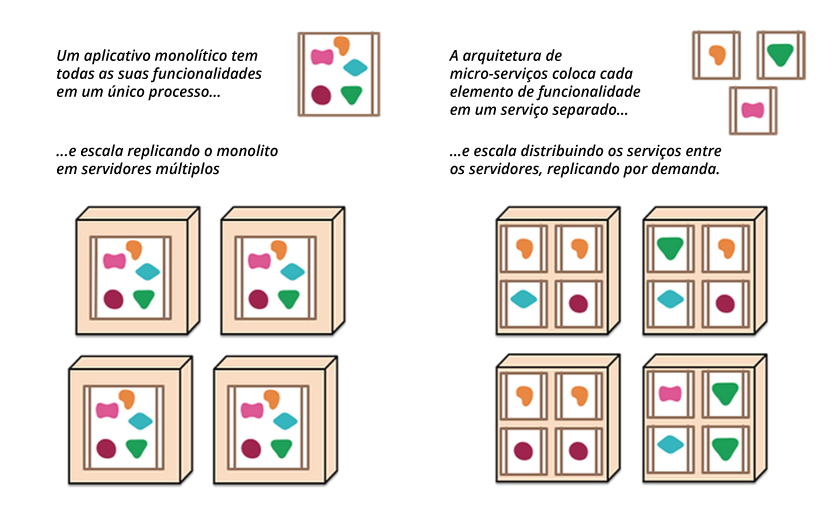
\includegraphics[width=0.8\linewidth]{imagens/1-arquitetura-microsservicos-fowler.png}    
    {\par \raggedright \footnotesize Fonte: \textcite{fowler_microsservicos_2022}\par}
\end{figure}

A arquitetura de microsserviços representa, portanto, um avanço em relação aos sistemas monolíticos tradicionais, promovendo a divisão dos serviços. Cada serviço possui sua própria base de dados, resultando na distribuição de dados por toda a arquitetura. De forma detalhada,conforme o entendimento de \textcite{lewis_microservices_2014}, enquanto o modelo monolítico centraliza tudo em um único bloco, a arquitetura de microsserviços distribui as responsabilidades em vários componentes menores e independentes. Essa abordagem promove escalabilidade, flexibilidade e resiliência em sistemas complexos e modernos.

A comunicação entre microsserviços, como já mencionado, ocorre predominantemente via \gls{api}s, \gls{http}, ou sistemas de mensagens assíncronas. A qualidade do design de comunicação é, portanto, determinante para a integração eficiente e a robustez do sistema, impactando diretamente o desempenho e a confiabilidade da solução. Proteger o tráfego de dados entre os serviços é essencial para assegurar a escalabilidade e a autonomia do sistema, além de atender às exigências rigorosas do setor econômico. Nesse contexto, é imprescindível adotar práticas de orquestração, monitoramento e documentação para visibilidade e controle sobre o comportamento dos serviços.

\subsection{Orquestração de Microsserviços}

Em arquiteturas de microsserviços, a \textbf{orquestração} refere-se à coordenação e gestão do ciclo de vida de múltiplos serviços independentes que colaboram para executar uma funcionalidade de negócio complexa \cite{newman_building_2022}. Em um sistema distribuído, como no nosso cenário de um assistente virtual multimodal, diferentes microsserviços precisam interagir de forma sequencial e eficiente. A escolha da tecnologia de orquestração é crucial para o desempenho, a latência e a resiliência do sistema. Este processo envolve a definição de como os serviços se comunicam, como os dados são serializados e como as chamadas são gerenciadas para garantir a entrega da funcionalidade completa ao usuário. A complexidade dos padrões de comunicação pode crescer exponencialmente com a adição de novos serviços, tornando o gerenciamento do sistema mais desafiador \cite{kleppmann_designing_2017}.

A orquestração eficaz é vital para mitigar os desafios inerentes aos microsserviços, como a complexidade de comunicação, a consistência de dados e a tolerância a falhas. Embora existam diversos protocolos de comunicação para sistemas distribuídos, desde comunicações tradicionais como WebSockets e Filas de Mensagens (MQTT) até soluções mais modernas como Apache Kafka\footnote{Disponível em https://kafka.apache.org. Acesso em 30/07/2025}, \acrshort{graphql}\footnote{Disponível em  https://graphql.org. Acesso em 30/07/2025} e Protocol Buffers, esta pesquisa concentra-se em três tecnologias que representam diferentes paradigmas arquiteturais e possuem sólida adoção na indústria\cite{jetbrains_state_2024}. A seleção de \gls{rest}, \gls{grpc} e Apache Thrift baseia-se em critérios específicos: (1) \gls{rest} representa o padrão consolidado e amplamente adotado em \gls{api}s web; (2) \gls{grpc} representa a evolução moderna com serialização binária e \acrshort{http}/2; e (3) Apache Thrift oferece uma alternativa madura com foco em performance e interoperabilidade entre linguagens. Essa escolha permite uma análise comparativa abrangente que cobre tanto soluções já estabelecidas quanto tecnologias emergentes, trazendo \textit{insights} práticos para decisões arquiteturais em contextos reais. A \autoref{tab:2-protocolos} apresenta uma comparação desses três protocolos de comunicação que serão avaliados nesse estudo, destacando suas características principais no contexto de comunicação e detalhando cada uma nas seções a seguir.

\begin{table}[H]
\caption{Comparativo de Protocolos de Comunicação para Orquestração de Microsserviços}
\centering
\begin{tabularx}{\textwidth}{|X|c|c|c|}
\hline
\textbf{Característica} & \textbf{\gls{rest}} & \textbf{\gls{grpc}} & \textbf{Thrift} \\
\hline
Comunicação & \acrshort{http}/1.1, \acrshort{http}/2 & \acrshort{http}/2 & \acrshort{tcp} \\
\hline
Serialização & \acrshort{json}, \acrshort{xml} & Protocol Buffers & Formato binário próprio \\
\hline
Tipo & Requisição/Resposta & Streaming & Requisição/Resposta \\
\hline
Binário & Não binário & .proto & .thrift \\
\hline
\end{tabularx}
\label{tab:2-protocolos}
\vspace{-0.2cm}
{\raggedright \footnotesize Fonte: Elaborado pelo autor.\par}
\end{table}

\subsubsection{\acrfull{rest}}

\gls{rest} constitui um padrão de comunicação amplamente adotado para o desenvolvimento de \gls{api}s web, fundamentado nos princípios do protocolo \gls{http}. Sua popularidade deriva da simplicidade, diversidade e utilização de padrões web, que facilitam a integração e o consumo em diversas plataformas \cite{mozilla_rest_2023}. Para a orquestração de microsserviços, \gls{rest} emprega requisições \gls{http} (GET, POST, PUT, DELETE) com o intuito de interagir com recursos, frequentemente utilizando payloads no formato \acrshort{json}. A natureza stateless do \gls{rest} simplifica o design dos serviços, pois cada requisição contém todas as informações necessárias para seu processamento, favorecendo, portanto, a escalabilidade horizontal. Entretanto, essa abordagem pode induzir bloqueios nos serviços até que a resposta seja recebida e requer que cada serviço conheça a localização dos demais, frequentemente necessitando de mecanismos de descoberta de serviços. A serialização textual (\acrshort{json}) e a sobrecarga do protocolo \gls{http}/1.1 podem também resultar em aumento de latência e consumo de banda em cenários com grandes volumes de dados ou que demandam alta performance \cite{mozilla_rest_2023}.

\subsubsection{\acrfull{grpc}}

O \acrshort{grpc} é um \textit{framework} de \acrfull{rpc} de código aberto, desenvolvido pelo Google, que utiliza \acrshort{http}/2 como protocolo de transporte e \textit{Protocol Buffers} como formato de serialização de dados \cite{google_grpc_nodate}. Diferente do \acrshort{rest}, que é orientado a recursos, o \acrshort{grpc} é orientado a serviços e métodos, permitindo a definição de contratos de serviço rigorosos por meio de arquivos \texttt{.proto}. O compilador de \textit{Protocol Buffers} processa esses arquivos para gerar automaticamente código cliente e servidor - conhecidos como \textit{bindings} - em múltiplas linguagens de programação.

\begin{figure}[H]
    \caption{Fluxo de comunicação gRPC entre clientes (Go/Ruby) e um serviço gRPC.}
    \label{fig:2-grpc-fluxo}
    \centering
    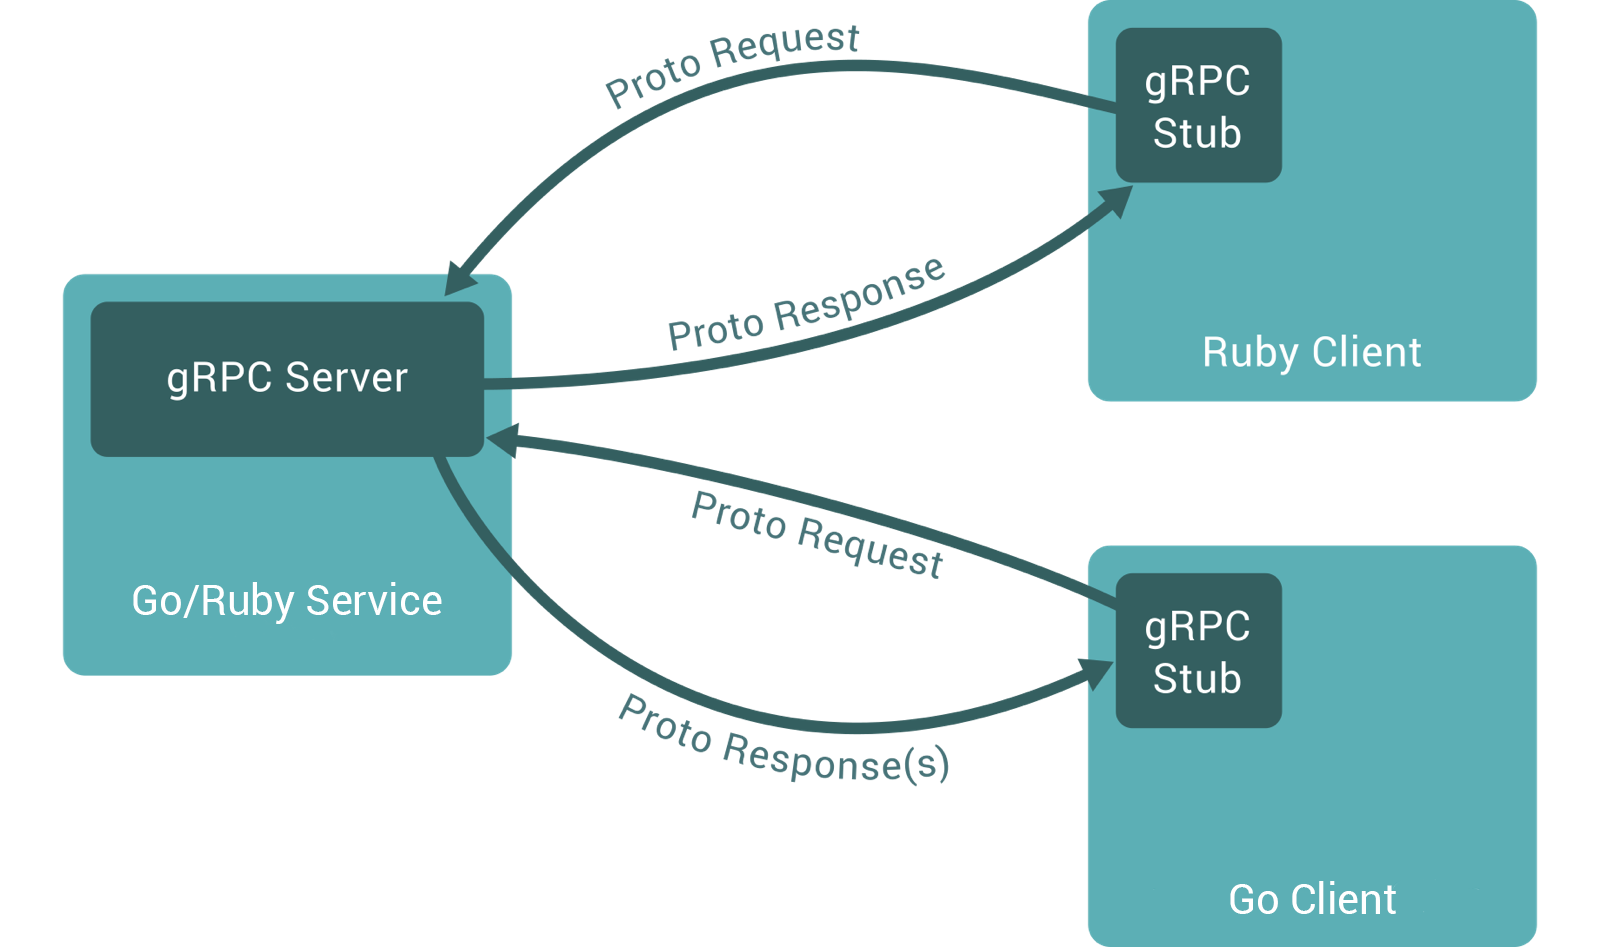
\includegraphics[width=0.5\linewidth]{imagens/2-gRPC-Flow.png}    
    {\par \raggedright \footnotesize Fonte: \textcite{google_grpc_nodate}.\par}
\end{figure}

Esses \textit{bindings} são fortemente tipados porque preservam toda a estrutura de dados e assinaturas de métodos definidas no contrato \texttt{.proto}, permitindo verificação de tipos em tempo de compilação e evitando erros comuns de serialização. A abordagem, combinada com a serialização binária e a multiplexação do \acrshort{http}/2, resulta em menor latência e maior \textit{throughput}, tornando-o ideal para comunicação interna entre microsserviços, nos quais a eficiência é importante. A geração automática de \textit{bindings multiplataforma} permite que serviços desenvolvidos em diferentes linguagens (como \textit{Go, Python, Java, C\#}) se comuniquem de forma transparente e eficiente, garantindo interoperabilidade em ambientes heterogêneos, conforme ilustrado na \autoref{fig:2-grpc-fluxo}. No entanto, o \acrshort{grpc} pode apresentar uma curva de aprendizado maior para clientes acostumados com \acrshort{rest} e possui uma especificação mais estrita, com menor suporte a outros tipos de conteúdo fora do \textit{Protobuf}.

\subsubsection{Apache Thrift}

O Apache Thrift é um \textit{framework} de \gls{rpc} e serialização de dados desenvolvido originalmente pelo Facebook e posteriormente incorporado ao ecossistema Apache. Sua arquitetura foi projetada especificamente para permitir comunicação eficiente entre serviços implementados em diferentes linguagens de programação \cite{apache_apache_nodate}.

A base do Thrift consiste em uma \textit{Interface Definition Language} (IDL) própria, onde os desenvolvedores definem os contratos de serviço em arquivos .thrift. Esses arquivos descrevem estruturas de dados, interfaces de serviço e exceções de forma independente de linguagem. O compilador Thrift então gera automaticamente o código correspondente na linguagem-alvo, produzindo \textit{bindings} fortemente tipados que garantem segurança e consistência na comunicação entre os serviços.

Assim como o \gls{grpc}, o Thrift emprega serialização binária para eficiência no transporte de dados, mas difere em sua abordagem de transporte, suportando tanto HTTP quanto TCP puro. Essa flexibilidade permite otimizações específicas para diferentes cenários de uso. O framework é particularmente adequado para ambientes heterogêneos onde serviços escritos em linguagens distintas (como Java, Python, C++, Ruby) precisam se comunicar com desempenho próximo ao de chamadas locais.

Entre suas principais vantagens destacam-se a baixa sobrecarga (\textit{overhead}) na serialização, suporte a tipos de dados complexos e a capacidade de trabalhar com conexões persistentes. No contexto de microsserviços, o Thrift se mostra uma alternativa robusta para cenários que exigem baixa latência e alta vazão, especialmente em implementações onde o controle fino sobre a camada de transporte é necessário \cite{apache_apache_nodate}.

\subsection{Desempenho e Escalabilidade}

O desempenho de um sistema refere-se à capacidade de responder de forma rápida e eficiente às solicitações dos usuários. Em arquiteturas de microsserviços, essa performance é impactada pela comunicação entre os serviços. O acoplamento solto da arquitetura permite o dimensionamento autônomo de cada serviço, distribui a carga de trabalho e reduz gargalos. Dessa forma, é possível aplicar técnicas como caching, balanceamento de carga e otimização dos tempos de resposta, fundamentos para manter o sistema responsivo sob alta demanda \cite{newman_building_2022}.

Em sistemas distribuídos, a latência da rede na comunicação entre serviços é um fator crítico. Para mitigar esse impacto e aproveitar plenamente os benefícios de sistemas resilientes e de baixa latência, é crucial investir em um design cuidadoso das interfaces e na implementação de mecanismos de resiliência, como circuit breakers, que monitoram falhas e, ao detectarem uma taxa elevada de erros, interrompem temporariamente as requisições ao serviço problemático. Essa abordagem evita falhas em cascata e permite a recuperação do serviço \cite[p. 131]{kleppmann_designing_2017}. 

A escalabilidade, por sua vez, é definida como a capacidade de um sistema crescer e se adaptar ao aumento da demanda \cite[p. 60]{fowler_microsservicos_2022}, e é um dos pilares que impulsionam a adoção de microsserviços. Conforme \cite{newman_building_2022}, a arquitetura de microsserviços facilita a escalabilidade horizontal, permitindo a adição ou remoção de instâncias de um serviço específico em resposta à demanda, em vez de replicar toda a aplicação. Essa granularidade assegura uma utilização de recursos mais eficiente e econômica, especialmente em ambientes de nuvem. A combinação de escalabilidade, resiliência e desempenho otimizado torna a arquitetura de microsserviços um modelo robusto para sistemas complexos e dinâmicos, como as aplicações no setor financeiro.
\vspace{\fill}
\subsection{Observabilidade e Monitoramento}

A arquitetura de microsserviços, embora traga benefícios significativos em flexibilidade e escalabilidade, introduz uma complexidade inerente devido à natureza distribuída e interconectada de seus componentes. Nesse cenário, a observabilidade e o monitoramento tornam-se cruciais para garantir a resiliência e a disponibilidade dos sistemas, especialmente em ambientes de alta criticidade como o setor financeiro \cite{arditti_microsservicos_2025}. A observabilidade pode ser definida como a capacidade de inferir o estado interno de um sistema a partir de seus dados externos, permitindo compreender e diagnosticar seu comportamento de forma eficaz. Práticas robustas de monitoramento, por sua vez, possibilitam a detecção rápida de problemas, como falhas de serviço, lentidão e sobrecarga, favorecendo respostas ágeis e a manutenção da estabilidade operacional \cite[p. 156]{fowler_microsservicos_2022}

Para alcançar uma observabilidade abrangente em microsserviços, é fundamental coletar e analisar três pilares de telemetria: métricas, logs e rastreamento distribuído. Métricas fornecem dados quantitativos sobre o desempenho do sistema (ex: utilização de CPU, memória, latência, throughput), enquanto os logs registram eventos e estados dos serviços, sendo essenciais para depuração e auditoria. O rastreamento distribuído, por sua vez, permite acompanhar o fluxo completo de uma requisição através de múltiplos microsserviços, identificando gargalos e falhas em cadeias de execução complexas  \cite{ibm_o_2023}. Ferramentas como Prometheus\footnote{Disponível em: \url{https://prometheus.io/}. Acesso em: 17 de jul. 2025.} e Grafana\footnote{Disponível em: \url{https://grafana.com/}. Acesso em: 17 de jul. 2025.} para métricas, o Elastick Stack\footnote{Disponível em: \url{https://www.elastic.co/elastic-stack/}. Acesso em: 17 de jul. 2025.} para logs e Jaeger\footnote{Disponível em: \url{https://www.jaegertracing.io/}. Acesso em: 17 de jul. 2025.} ou Zipkin\footnote{Disponível em: \url{https://zipkin.io/}. Acesso em: 17 de jul. 2025.} para rastreamento distribuído são comumente empregadas para consolidar e visualizar esses dados.

No contexto do mercado financeiro, a observabilidade inteligente é vital para prevenir problemas e proteger operações sensíveis, onde a integridade e a agilidade são indispensáveis. Um monitoramento preciso e em tempo real da stack de microsserviços garante que nenhuma métrica ou rastreamento importante seja perdido, fornecendo informações gerenciais precisas às equipes de DevOps e aumentando o tempo de resposta para prevenção e triagem de incidentes \cite{baumgartner_observabilidade_2024}.